\documentclass[tikz,border=1mm]{standalone}
\usetikzlibrary{matrix,chains,positioning,decorations.pathreplacing,arrows}

% Code modified from here https://tex.stackexchange.com/questions/505741/architecture-neural-network-with-weights

\begin{document}
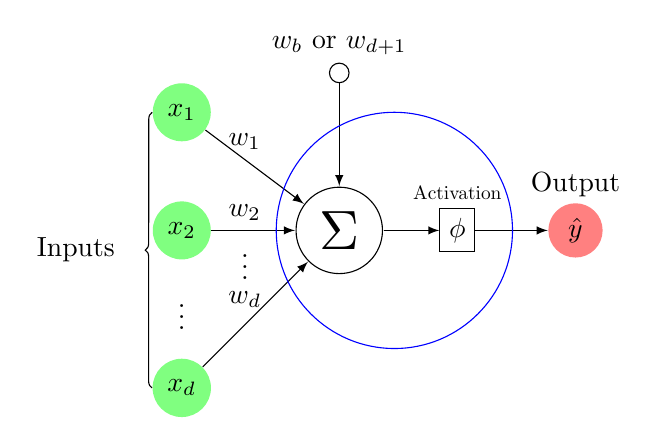
\begin{tikzpicture}[>=latex]
\path
(0,0)     node[circle,draw,scale=2,inner sep=2pt] (S) {$\Sigma$}
+(90:2) node[circle,draw,inner sep=2.5pt] (b) {}
          node[above=1mm] {$w_b$ or $w_{d+1}$}
+(-2,1.5)  node[circle,fill=green!50]  (x1) {$x_1$}
+(-2,0)    node[circle,fill=green!50]  (x2) {$x_2$}
+(-2,-1) node  ()  {$\vdots$}
+(-2,-2) node[circle,fill=green!50]  (xd) {$x_d$}
(1.5,0)    node[draw] (h) {$\phi$} node[above=3mm, scale=.7]{Activation}
+(0:1.5)  node[circle,fill=red!50]  (y1) {$\hat{y}$} node[above=3mm]() {Output};

% +(-15:3) node[circle,fill=red!50]  (y2) {$\hat{y}_2$};
\draw[->] (S)--(h);
\draw[->] (b)--(S);
\draw[->] (h)--(y1); % node[pos=.6,above]{$w_1$};
% \draw[->] (g)--(y2) node[pos=.6,below]{$\omega_{2,1}^{(3)}$};
\draw[->] (x1)--(S) node[pos=.4,above]{$w_1$};
\draw[->] (x2)--(S) node[pos=.4,above]{$w_2$}; 
\draw[->] (xd)--(S) node[pos=.4,above=1mm]{$w_d$} node[pos=.4,above=4.5mm]{$\vdots$};
\draw[blue] (0.7,0) circle(1.5);
\draw[decorate,decoration={brace,mirror}] (x1.west) -- node[left=10pt] {Inputs} (xd.west);
\end{tikzpicture}
\end{document}
